%! TEX root = main.tex
One particular question we would like to investigate is the relationship between training loss and the actual prediction errors or accuracy.
As we have seen from the previous section, further training in many cases only reduces the IC losses, while the PDE losses already converged.
Reductions in IC losses, though improve the prediction error of solution at $t=0$, do not help the overall spatial-temporal $L_{2,sp-t}$ at all.
It implies the training loss may not reflect the models' prediction capabilities.
If true, then the aggregated loss is not a proper indicator to monitor the training progress.
Also, given a known aggregated loss and error, we may not able to predict how much loss we need to further reduce to achieve a desired error level.
We would hence like to investigate the relationship between the aggregated loss and the overall spatial-temporal errors.

Figure \ref{fig:tgv2d-re100-err-vs-loss} shows the $L_{2,sp-t}$ of all cases.
The $x$-axis represents the square roots of aggregate losses, and the $y$-axis is $L_{2,sp-t}$ of $u$ and $v$.
For each case, $u$ and $v$ are separate dots in the figure.
The figure uses the square roots of aggregate losses because losses are defined as the sum of residuals' squares.
See equation \eqref{eq:residual-norms}

\begin{figure}[hbt!]
    \centering%
    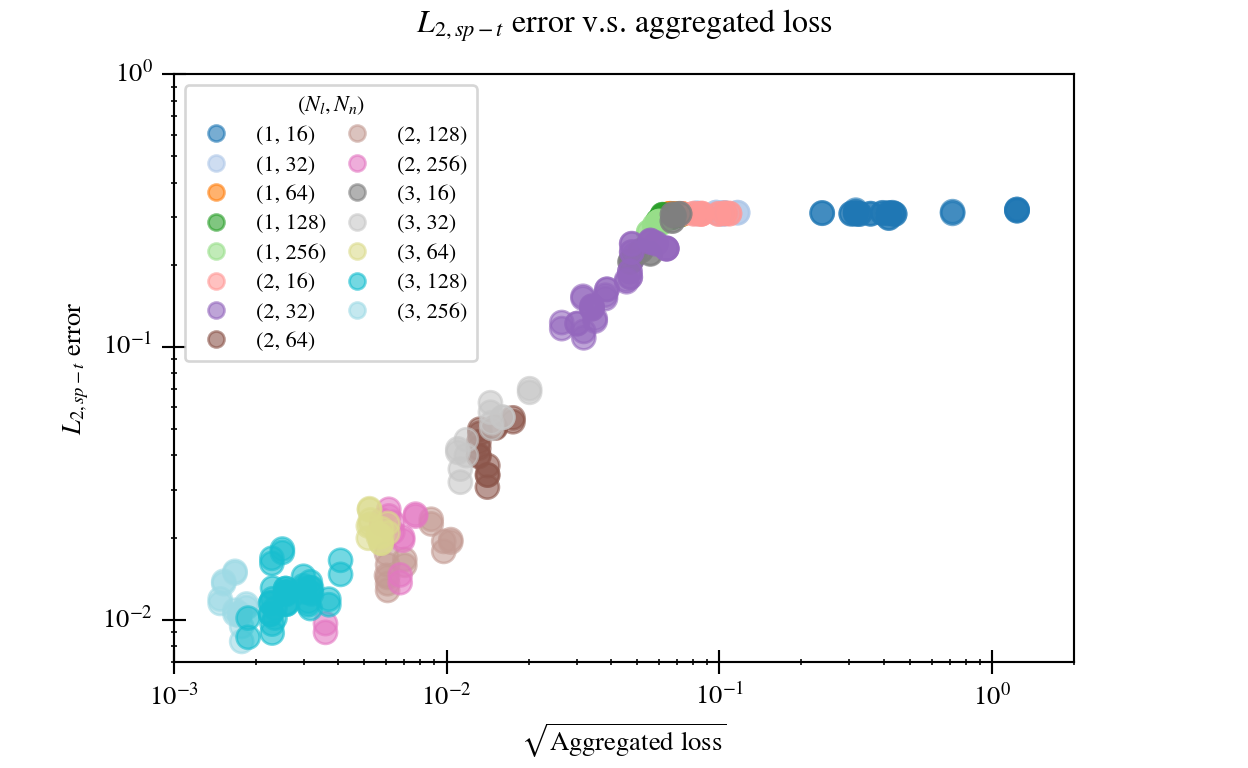
\includegraphics[width=0.9\linewidth]{tgv-2d-re100/err-vs-loss/err-loss.png}
    \caption[%
        PINNs, 2D TGV, $Re=100$: $L_{2,sp-t}$ error v.s. aggregated loss%
    ]{%
        PINNs, 2D TGV, $Re=100$: $L_{2,sp-t}$ error v.s. aggregated loss.%
        $L_{2,sp-t}$ errors for $u$ and $v$ from the same case are separate data points in the figure.
    }
    \label{fig:tgv2d-re100-err-vs-loss}
\end{figure}

From the figure, the first observation is the flat region in the top-right corner.
It says, for these cases, the aggregated loss is completely dominated by IC losses.
These cases are majorly those with only one hidden layer, implying that one hidden layer may not be enough to approximate the solutions of the Navier-Stokes equations.

Although the relationship is approximately linear in the middle range, the data points become more diversed in the bottom-left corner.
And a similar loss level has a wider range of possible $L_{2,sp-t}$.
Given the observed trends, it is reasonable to suspect that, if we have more data further extend to the left of this figure, the possible $L_{2,sp-t}$ corresponding to a loss level may have wider and wider range, meaning it is more difficult to predict the solution accuracy for a given training loss.

In addition, we suspect that using adaptive loss weighting like annealing loss aggregation may even complicate the problem.
As each loss term's weight is updated according to the ratio of characteristic gradient magnitudes, it is likely that two iterations have the same level of aggregated losses but have different prediction accuracies. 
This observation somehow hurts the predictability of PINNs.
Especially when dealing with real-world problems where we don't have exact solutions to calculate the errors, the losses may be the only indicator for us to know a model's prediction capability.
If lowering the loss does not improve the prediction accuracy, we have no means to know if training should keep going.
% vim:ft=tex